\chapter{Benchmarking and Results}\label{ch:results}
To finish the objective of this thesis at last a setting needs to be built where these algorithms are used for \ac{IPC} over shared memory. This setting was also used to benchmark the performance of these algorithms to identify the best performing wait-free algorithms that can be used. In the \cite{githubMA} the folder benches includes the setting and benchmark of these algorithms. As seen before these algorithms were divided into 4 categories, \ac{MPMC}, \ac{MPSC}, \ac{SPMC} and \ac{SPSC}. Therefore 4 different \ac{IPC} over shared memory settings were built to analyse firstly if all algorithms work as intended and secondly to compare the performance of all algorithms. Even though \ac{SPMC} category only has one algorithm, the built setting was still interesting to check and validate if the algorithm works as intended. After identifying the best algorithm 3 more settings were built. One setting was to see if the \ac{SPMC} queue or the best performing queues of the other categories would be faster for the \ac{SPSC} category. The same was done for the \ac{MPSC} category by checking if the best \ac{MPMC} queue or the best \ac{MPSC} queue would perform better. Finally for the \ac{SPMC} category the same was done to check if the best \ac{MPMC} or \ac{SPMC} queue would be better. The best \ac{SPSC} queue could not be tested for higher producer or consumer numbers, since the missing helping structures and missing atomic primitives would lead to deadlocks or inconsistent data. The benchmarks were done on a system with an Intel i7-12700H x86 processor with 14 cores. The benchmarks were implemented with the help of the \texttt{criterion} crate, which is a benchmarking library for Rust. This chapter will show in general how the benchmark settings were implemented to understand the results later.

\section{Benchmark Structure}
All benchmarks follow a consistent architecture to ensure fair comparison between queue implementations. The benchmarks measure the time taken for producers and consumers to exchange a fixed number of items through each queue implementation using \ac{IPC} over shared memory. This section explains the general benchmark structure using the \ac{MPMC} benchmark as a representative example, as the same patterns apply to all queue categories. Not every line will be explained, but the most important lines will be explained to understand the general structure of the benchmarks. 

\subsection{Benchmark Parameters and Configuration}
Before examining the benchmark implementation details, it is important to understand the benchmark parameters that control the test scenarios. These constants define the scale and scope of the performance measurements, as shown in \cref{lst:bench-constants}.

\begin{lstlisting}[language=Rust, style=boxed, caption={Benchmark configuration constants}, label={lst:bench-constants}]
const ITEMS_PER_PROCESS_TARGET: usize = 170_000;
const PROCESS_COUNTS_TO_TEST: &[(usize, usize)] = &[(1, 1), (2, 2), (4, 4), (6, 6)];
const MAX_BENCH_SPIN_RETRY_ATTEMPTS: usize = 100_000_000_000;
\end{lstlisting}

Line 1 sets the number of items each producer process will generate. The value of 170,000 items provides sufficient workload to measure performance while keeping individual benchmark runs reasonable in duration. Line 2 defines the producer and consumer configurations to test as tuples. The array \texttt{[(1, 1), (2, 2), (4, 4), (6, 6)]} tests symmetric configurations from single producer and single consumer up to 6 producers and 6 consumers, allowing analysis of scalability. Line 3 sets the maximum spin attempts before considering an operation failed. This large value ensures that wait-free operations have sufficient opportunity to complete.

For other benchmark categories, these constants are adjusted appropriately. For example, the \ac{MPSC} benchmark uses:

\begin{lstlisting}[language=Rust, style=boxed, caption={MPSC-specific configuration}, label={lst:mpsc-constants}]
const ITEMS_PER_PRODUCER_TARGET: usize = 500_000;
const PRODUCER_COUNTS_TO_TEST: &[usize] = &[1, 2, 4, 8, 14];
\end{lstlisting}

The \ac{MPSC} configuration tests up to 14 producers with a single consumer, using more items per producer to ensure the consumer remains busy throughout the benchmark. Similarly, \ac{SPMC} and \ac{SPSC} benchmarks have their own tailored parameters to effectively measure their specific use-cases.

\subsection{Benchmark Interface Implementation}
Each queue implementation must provide a uniform interface for benchmarking. This is achieved through a common trait that abstracts the queue-specific operations, as shown in \cref{lst:bench-trait}. The following pop and push traits implement the dequeue and enqueue operations respectively for the queues.

\begin{lstlisting}[language=Rust, style=boxed, caption={Benchmark trait for MPMC queues}, label={lst:bench-trait}]
trait BenchMpmcQueue<T: Send + Clone>: Send + Sync + 'static {
    fn bench_push(&self, item: T, process_id: usize) -> Result<(), ()>;
    fn bench_pop(&self, process_id: usize) -> Result<T, ()>;
    fn bench_is_empty(&self) -> bool;
    fn bench_is_full(&self) -> bool;
}

// Example implementation for YangCrummeyQueue
impl<T: Send + Clone + 'static> BenchMpmcQueue<T> for YangCrummeyQueue<T> {
    fn bench_push(&self, item: T, process_id: usize) -> Result<(), ()> {
        self.enqueue(process_id, item)
    }

    fn bench_pop(&self, process_id: usize) -> Result<T, ()> {
        self.dequeue(process_id)
    }

    fn bench_is_empty(&self) -> bool {
        self.is_empty()
    }

    fn bench_is_full(&self) -> bool {
        false  // YangCrummeyQueue has unbounded capacity
    }
}
\end{lstlisting}

The trait in lines 1 to 6 defines a common interface that all \ac{MPMC} queues must implement. The \texttt{process\_id} parameter in lines 2 and 3 allows queues to distinguish between different processes, which is necessary for some algorithms. Lines 9 to 24 show how the \ac{YMC} queue maps its specific methods to the common interface. The \texttt{bench\_is\_full} method in line 23 returns false for queues with unbounded capacity. This mapping is done for all queues in the respective categories, so that the benchmarks can be run with all queues without changing the benchmark code to compare fairly.

\subsection{Process Synchronisation Infrastructure}
Benchmarking concurrent algorithms requires careful synchronisation to ensure all processes start simultaneously and coordinate their completion for fair comparisons. Two synchronisation structures manage this coordination, as shown in \cref{lst:sync-structures}.

\begin{lstlisting}[language=Rust, style=boxed, caption={Process synchronisation structures}, label={lst:sync-structures}]
#[repr(C)]
struct MpmcStartupSync {
    producers_ready: AtomicU32,
    consumers_ready: AtomicU32,
    go_signal: AtomicBool,
}

impl MpmcStartupSync {
    fn new_in_shm(mem_ptr: *mut u8) -> &'static Self {
        let sync_ptr = mem_ptr as *mut Self;
        unsafe {
            ptr::write(
                sync_ptr,
                Self {
                    producers_ready: AtomicU32::new(0),
                    consumers_ready: AtomicU32::new(0),
                    go_signal: AtomicBool::new(false),
                },
            );
            &*sync_ptr
        }
    }

    fn shared_size() -> usize {
        std::mem::size_of::<Self>()
    }
}

#[repr(C)]
struct MpmcDoneSync {
    producers_done: AtomicU32,
    consumers_done: AtomicU32,
    total_consumed: AtomicUsize,
}
\end{lstlisting}

The \texttt{MpmcStartupSync} structure in lines 1 to 6 coordinates the startup phase. Producers increment \texttt{producers\_ready} in line 3 when ready, consumers increment \texttt{consumers\_ready} in line 4, and all processes wait for \texttt{go\_signal} in line 5 before starting. The \texttt{new\_in\_shm} method in lines 9 to 22 initialises the structure directly in shared memory using placement new. The \texttt{MpmcDoneSync} structure in lines 29 to 34 tracks completion, with \texttt{total\_consumed} in line 33 which is used to verify that no items were lost during the benchmark.

\subsection{Benchmark Execution Framework}

The core benchmark logic is implemented in a generic function that handles process creation, execution, and measurement, as demonstrated in \cref{lst:fork-and-run}.

\begin{lstlisting}[language=Rust, style=boxed, caption={Generic benchmark execution function}, label={lst:fork-and-run}]
fn fork_and_run_mpmc_with_helper<Q, F>(
    queue_init_fn: F,
    num_producers: usize,
    num_consumers: usize,
    items_per_process: usize,
    needs_helper: bool,
) -> Duration
where
    Q: BenchMpmcQueue<usize> + 'static,
    F: FnOnce() -> (&'static Q, *mut u8, usize),
{
    let total_items = num_producers * items_per_process;
    
    // Initialise queue in shared memory
    let (q, q_shm_ptr, q_shm_size) = queue_init_fn();
    
    // Allocate synchronisation structures
    let startup_sync_size = MpmcStartupSync::shared_size();
    let startup_sync_shm_ptr = unsafe { map_shared(startup_sync_size) };
    let startup_sync = MpmcStartupSync::new_in_shm(startup_sync_shm_ptr);
    
    let mut producer_pids = Vec::with_capacity(num_producers);
    let mut consumer_pids = Vec::with_capacity(num_consumers);
    
    // Fork producer processes
    for producer_id in 0..num_producers {
        match unsafe { fork() } {
            Ok(ForkResult::Child) => {
                // Signal ready and wait for go signal
                startup_sync.producers_ready.fetch_add(1, Ordering::AcqRel);
                while !startup_sync.go_signal.load(Ordering::Acquire) {
                    std::hint::spin_loop();
                }
                
                // Produce items
                for i in 0..items_per_process {
                    let item_value = producer_id * items_per_process + i;
                    while q.bench_push(item_value, producer_id).is_err() {
                        std::hint::spin_loop();
                    }
                }
                
                unsafe { libc::_exit(0) };
            }
            Ok(ForkResult::Parent { child }) => {
                producer_pids.push(child);
            }
            Err(e) => panic!("Fork failed: {}", e),
        }
    }
    
    // Wait for all processes to be ready
    while startup_sync.producers_ready.load(Ordering::Acquire) < num_producers as u32
        || startup_sync.consumers_ready.load(Ordering::Acquire) < num_consumers as u32
    {
        std::hint::spin_loop();
    }
    
    // Start timing and signal processes to begin
    let start_time = std::time::Instant::now();
    startup_sync.go_signal.store(true, Ordering::Release);
    
    // Wait for completion
    for pid in producer_pids {
        waitpid(pid, None).expect("waitpid failed");
    }
    
    start_time.elapsed()
}
\end{lstlisting}

The function signature in lines 1 to 10 accepts a queue initialisation function and benchmark parameters. The \texttt{needs\_helper} parameter in line 6 supports queues like Verma's that require a helper thread. Line 15 initialises the queue using the provided function, which returns the queue reference and shared memory details. Lines 26 to 50 show the producer process creation where line 30 signals readiness, lines 31 to 33 implement ensures that every process waits for the go signal, and lines 36 to 41 produce items with retry logic. Lines 53 to 57 ensure all processes are ready before starting. Line 60 captures the start time immediately before signalling processes to begin in line 61. Lines 64 to 66 wait for all producer processes to complete before calculating the elapsed time in line 68.

\subsection{Queue-Specific Benchmark Integration}

Each queue type requires a specific benchmark function that integrates with the Criterion framework, as shown in \cref{lst:queue-benchmark}.

\begin{lstlisting}[language=Rust, style=boxed, caption={Queue-specific benchmark function}, label={lst:queue-benchmark}]
fn bench_yang_crummey(c: &mut Criterion) {
    let mut group = c.benchmark_group("YangCrummeyMPMC_");

    for &(num_prods, num_cons) in PROCESS_COUNTS_TO_TEST {
        let items_per_process = ITEMS_PER_PROCESS_TARGET;
        let total_processes = num_prods + num_cons;

        group.bench_function(
            format!("{}P_{}C", num_prods, num_cons),
            |b: &mut Bencher| {
                b.iter_custom(|_iters| {
                    fork_and_run_mpmc_with_helper::<YangCrummeyQueue<usize>, _>(
                        || {
                            // Calculate required shared memory size
                            let bytes = YangCrummeyQueue::<usize>::shared_size(total_processes);
                            let shm_ptr = unsafe { map_shared(bytes) };
                            
                            // Initialise queue in shared memory
                            let q = unsafe {
                                YangCrummeyQueue::init_in_shared(shm_ptr, total_processes)
                            };
                            
                            (q, shm_ptr, bytes)
                        },
                        num_prods,
                        num_cons,
                        items_per_process,
                        false,  // YangCrummey doesn't need helper
                    )
                })
            },
        );
    }

    group.finish();
}
\end{lstlisting}

Line 2 creates a benchmark group with a descriptive name. Line 4 iterates through different producer/consumer configurations from the constant array \texttt{PROCESS\_COUNTS\_TO\_TEST}. Line 9 formats the benchmark name to indicate the configuration. Lines 11 to 30 use Criterion's \texttt{iter\_custom} method to measure custom timing, as the benchmark itself measures process execution time. The closure in lines 13 to 23 initialises the queue where line 15 calculates the exact shared memory size needed and line 16 allocates the shared memory region. After that lines 19 to 21 initialise the queue at the allocated address.

\subsection{Consumer Process Implementation}
The consumer processes follow a similar pattern but with additional logic to handle termination and verify correctness, as shown in \cref{lst:consumer-process}.

\begin{lstlisting}[language=Rust, style=boxed, caption={Consumer process implementation}, label={lst:consumer-process}]
// Fork consumer processes
for consumer_id in 0..num_consumers {
    match unsafe { fork() } {
        Ok(ForkResult::Child) => {
            startup_sync.consumers_ready.fetch_add(1, Ordering::AcqRel);

            while !startup_sync.go_signal.load(Ordering::Acquire) {
                std::hint::spin_loop();
            }

            let mut consumed_count = 0;
            let target_items = total_items / num_consumers;
            let extra_items = if consumer_id < (total_items % num_consumers) {
                1
            } else {
                0
            };
            let my_target = target_items + extra_items;

            let mut consecutive_empty_checks = 0;
            const MAX_CONSECUTIVE_EMPTY_CHECKS: usize = 40000;

            while consumed_count < my_target {
                match q.bench_pop(num_producers + consumer_id) {
                    Ok(_item) => {
                        consumed_count += 1;
                        consecutive_empty_checks = 0;
                    }
                    Err(_) => {
                        if done_sync.producers_done.load(Ordering::Acquire)
                            == num_producers as u32
                        {
                            consecutive_empty_checks += 1;

                            if consecutive_empty_checks > MAX_CONSECUTIVE_EMPTY_CHECKS {
                                break;  // Queue likely empty
                            }
                        }
                        
                        // Backoff strategy
                        for _ in 0..100 {
                            std::hint::spin_loop();
                        }
                    }
                }
            }

            done_sync
                .total_consumed
                .fetch_add(consumed_count, Ordering::AcqRel);
            done_sync.consumers_done.fetch_add(1, Ordering::AcqRel);

            unsafe { libc::_exit(0) };
        }
        Ok(ForkResult::Parent { child }) => {
            consumer_pids.push(child);
        }
        Err(e) => panic!("Fork failed for consumer: {}", e),
    }
}
\end{lstlisting}

Lines 12 to 18 calculate each consumer's share of items, distributing any remainder among the first consumers. The main consumption loop in lines 23 to 46 implements a termination strategy where lines 25 to 27 reset the empty check counter on successful pop while lines 30 to 38 check if all producers have finished and implement a termination condition. Lines 48 to 51 atomically update the total consumed count for later verification. Line 53 uses \texttt{\_exit} to avoid cleanup that might interfere with shared memory.

\subsection{Validation}
After all producer and consumer processes complete, the benchmark validates that no items were lost or double read during the concurrent operations. This validation is important for ensuring the correctness of each queue implementation under \ac{IPC} scenarios, as shown in \cref{lst:result-validation}.

\begin{lstlisting}[language=Rust, style=boxed, caption={Post-benchmark validation of results}, label={lst:result-validation}]
// Wait for all processes to complete
for pid in producer_pids {
    waitpid(pid, None).expect("waitpid for producer failed");
}

for pid in consumer_pids {
    waitpid(pid, None).expect("waitpid for consumer failed");
}

let duration = start_time.elapsed();

// Validate that all items were consumed
let total_consumed = done_sync.total_consumed.load(Ordering::Acquire);

if total_consumed != total_items {
    eprintln!(
        "Warning (MPMC): Total consumed {}/{} items. Q: {}, Prods: {}, Cons: {}",
        total_consumed,
        total_items,
        std::any::type_name::<Q>(),
        num_producers,
        num_consumers
    );
}

// Clean up shared memory regions
unsafe {
    if !q_shm_ptr.is_null() {
        unmap_shared(q_shm_ptr, q_shm_size);
    }
    unmap_shared(startup_sync_shm_ptr, startup_sync_size);
    unmap_shared(done_sync_shm_ptr, done_sync_size);
}

duration
\end{lstlisting}

Lines 2 to 8 wait for all processes to complete before proceeding with validation. After that line 13 atomically reads the total number of items consumed across all consumer processes. The validation check in lines 15 to 24 compares the consumed count against the expected total. If items are missing, line 17 prints a detailed warning that includes the actual versus expected counts in line 18, the queue type name in line 20, and the producer and consumer configuration in lines 21 and 22. This warning helps identify queue implementations that may lose items under high contention or have synchronisation issues and to verify that the queue operates correctly under concurrent access, if the warning does not appear.

\subsection{Benchmark Configuration}
The benchmarks use Criterion's configuration options to ensure reliable measurements, as shown in \cref{lst:criterion-config}.

\begin{lstlisting}[language=Rust, style=boxed, caption={Criterion benchmark configuration}, label={lst:criterion-config}]
fn custom_criterion() -> Criterion {
    Criterion::default()
        .warm_up_time(Duration::from_secs(1))
        .measurement_time(Duration::from_secs(4200))
        .sample_size(500)
}

criterion_group! {
    name = benches;
    config = custom_criterion();
    targets =
        bench_wcq_queue,
        bench_turn_queue,
        bench_kogan_petrank_queue,
        bench_yang_crummey
}

criterion_main!(benches);
\end{lstlisting}

Line 3 sets a 1-second warm-up period to stabilise system state. Line 4 configures 4200 seconds of measurement time per benchmark. Line 5 sets 500 samples, as each sample involves creating multiple processes and produce and consume a set number of items. Lines 8 to 16 define the benchmark group with all queue implementations to test.

The same benchmark structure is applied to all benchmarks with appropriate modifications to the number of producers and consumers. This consistent approach ensures fair comparison across all implementations while accurately measuring their performance characteristics under \ac{IPC} scenarios.

\section{Benchmark Results}
The benchmark results are presented for each queue category, followed by cross-category comparisons to determine the optimal wait-free data structure for different contention scenarios. All measurements represent the mean execution time in microseconds ($\mu$s) for completing the configured workload across multiple samples. In every bench 500 samples were taken to have enough results to compare the performance. The amount of data produced and consumed was always different for each category. The queues inside each category were always tested with the same amount of data to ensure fair comparison. The amount of items used for each category is shown in the respective subsections.

\subsection{\acf{SPSC} Queue Performance}
The \ac{SPSC} benchmarks evaluated 11 different queue implementations with 35000000 items to ensure sufficient workload for accurate measurement. As shown in \cref{tab:spsc-results}, the \ac{BLQ} achieved the best performance with a mean execution time of 65199.6 $\mu$s.

\begin{table}[htb]
\centering
\caption{\ac{SPSC} Queue Performance Results (35000000 items)}
\label{tab:spsc-results}
\begin{tabular}{@{}lrr@{}}
\toprule
Queue Implementation & Mean Time ($\mu$s) & Relative Performance \\
\midrule
\ac{BLQ} & 65199.6 & 1.00x \\
\ac{IFFQ} & 124149.9 & 1.90x \\
\ac{LLQ} & 147800.2 & 2.27x \\
\ac{BIFFQ} & 159429.6 & 2.45x \\
\ac{FFQ} & 203053.4 & 3.11x \\
\ac{mSPSC} & 331283.6 & 5.08x \\
\ac{uSPSC} & 418840.0 & 6.42x \\
\ac{JPQ}'s \ac{SPSC} Variant & 626541.9 & 9.61x \\
Lamport's Queue & 957312.6 & 14.68x \\
B-Queue & 1552513.1 & 23.81x \\
\ac{dSPSC} & 2413354.7 & 37.02x \\
\bottomrule
\end{tabular}
\end{table}

The results reveal that the cache-aware algorithms (\ac{BLQ}, \ac{IFFQ}, \ac{LLQ}, \ac{BIFFQ}) are all faster than the other approaches, demonstrating the importance of cache optimisation. The \ac{BLQ}'s superior performance can be attributed to its additional batching mechanism, which amortises synchronisation costs across multiple operations while maintaining cache locality.

Notably, the dynamic allocation-based queues (\ac{dSPSC}, \ac{uSPSC}) showed worse performance, with \ac{dSPSC} being 37 times slower than \ac{BLQ}. This overhead stems from the memory pool management required for shared memory compatibility, as discussed in \cref{ch:implementation}.

\begin{figure}[htb]
\centering
\caption{Violin plot showing the distribution of execution times for \ac{SPSC} queue implementations and 35,000,000 total items)}
\label{fig:spsc-violin}
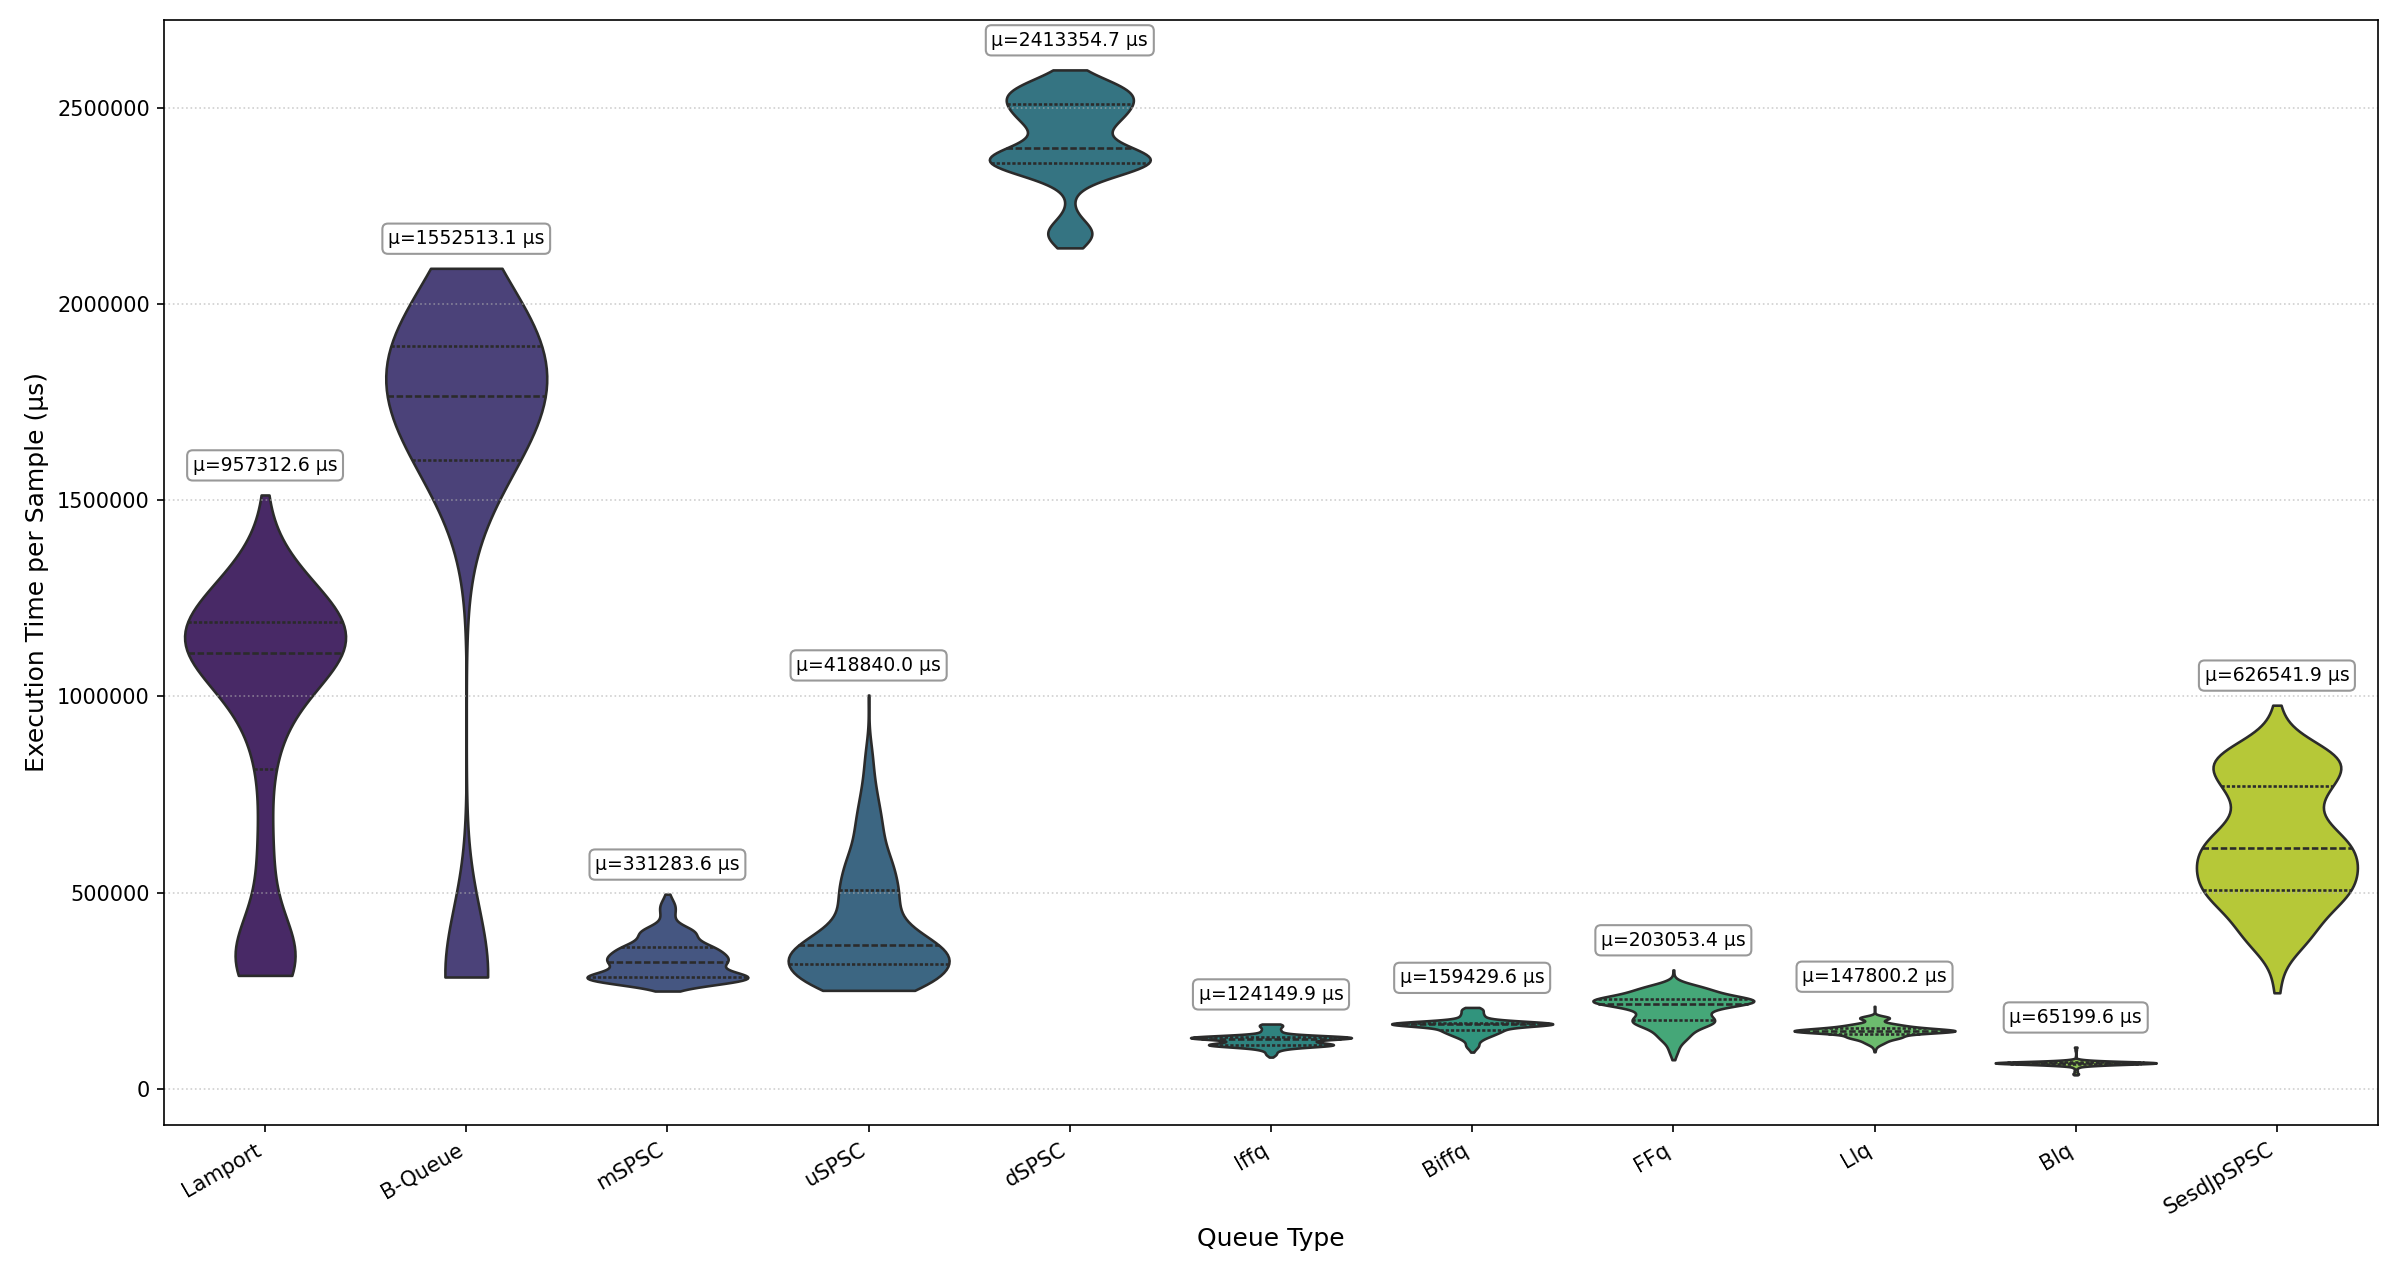
\includegraphics[width=\textwidth]{images/results/spsc_queue_performance_violin_test.png}
\end{figure}

The violin plot in \cref{fig:spsc-violin} illustrates the distribution of execution times across all SPSC implementations. It can be observed that the Lamport queue has no consistent performance with greatly varying results. It often achieves great execution times, but also often bad execution times. This is probably because of bad cache design of the queue that was talked about in \cref{alg:lamport-queue}. The \ac{BLQ} on the other hand shows not only the lowest median execution time but also the most consistent performance with minimal variance, which is an important trait to be able to design hard timing constraints for \ac{HRTS}. 

\subsection{\acf{MPSC} Queue Performance}
For \ac{MPSC} scenarios, four queue implementations were tested with varying producer counts from 1 to 14, each producer generating 500000 items. \cref{tab:mpsc-results} presents the mean performance across different producer configurations, which is visualised in \cref{fig:mpsc-mean-performance}. DQueue with a mean execution time of 13967.2 $\mu$s for 1 producer, 29039.9 $\mu$s for 2 producers, and scaling up to 323126.2 $\mu$s for 14 producers, outperformed all other implementations.

\begin{table}[htb]
\centering
\caption{\ac{MPSC} Queue Performance Results (500000 items per producer)}
\label{tab:mpsc-results}
\begin{tabular}{@{}lrrrrr@{}}
\toprule
Queue & 1P & 2P & 4P & 8P & 14P \\
\midrule
DQueue & 13967.2 & 29039.9 & 72894.1 & 170676.4 & 323126.2 \\
Drescher & 22932.0 & 89353.0 & 189703.0 & 434820.2 & 955047.8 \\
Jiffy & 32280.3 & 62159.1 & 126199.3 & 276401.5 & 538978.2 \\
\ac{JPQ}'s \ac{MPSC} Variant & 94912.5 & 252959.1 & 648641.6 & 2191529.2 & 4548422.3 \\
\bottomrule
\end{tabular}
\end{table}

\begin{figure}[htb]
\centering
\caption{Mean execution time of MPSC queue implementations as producer count increases}
\label{fig:mpsc-mean-performance}
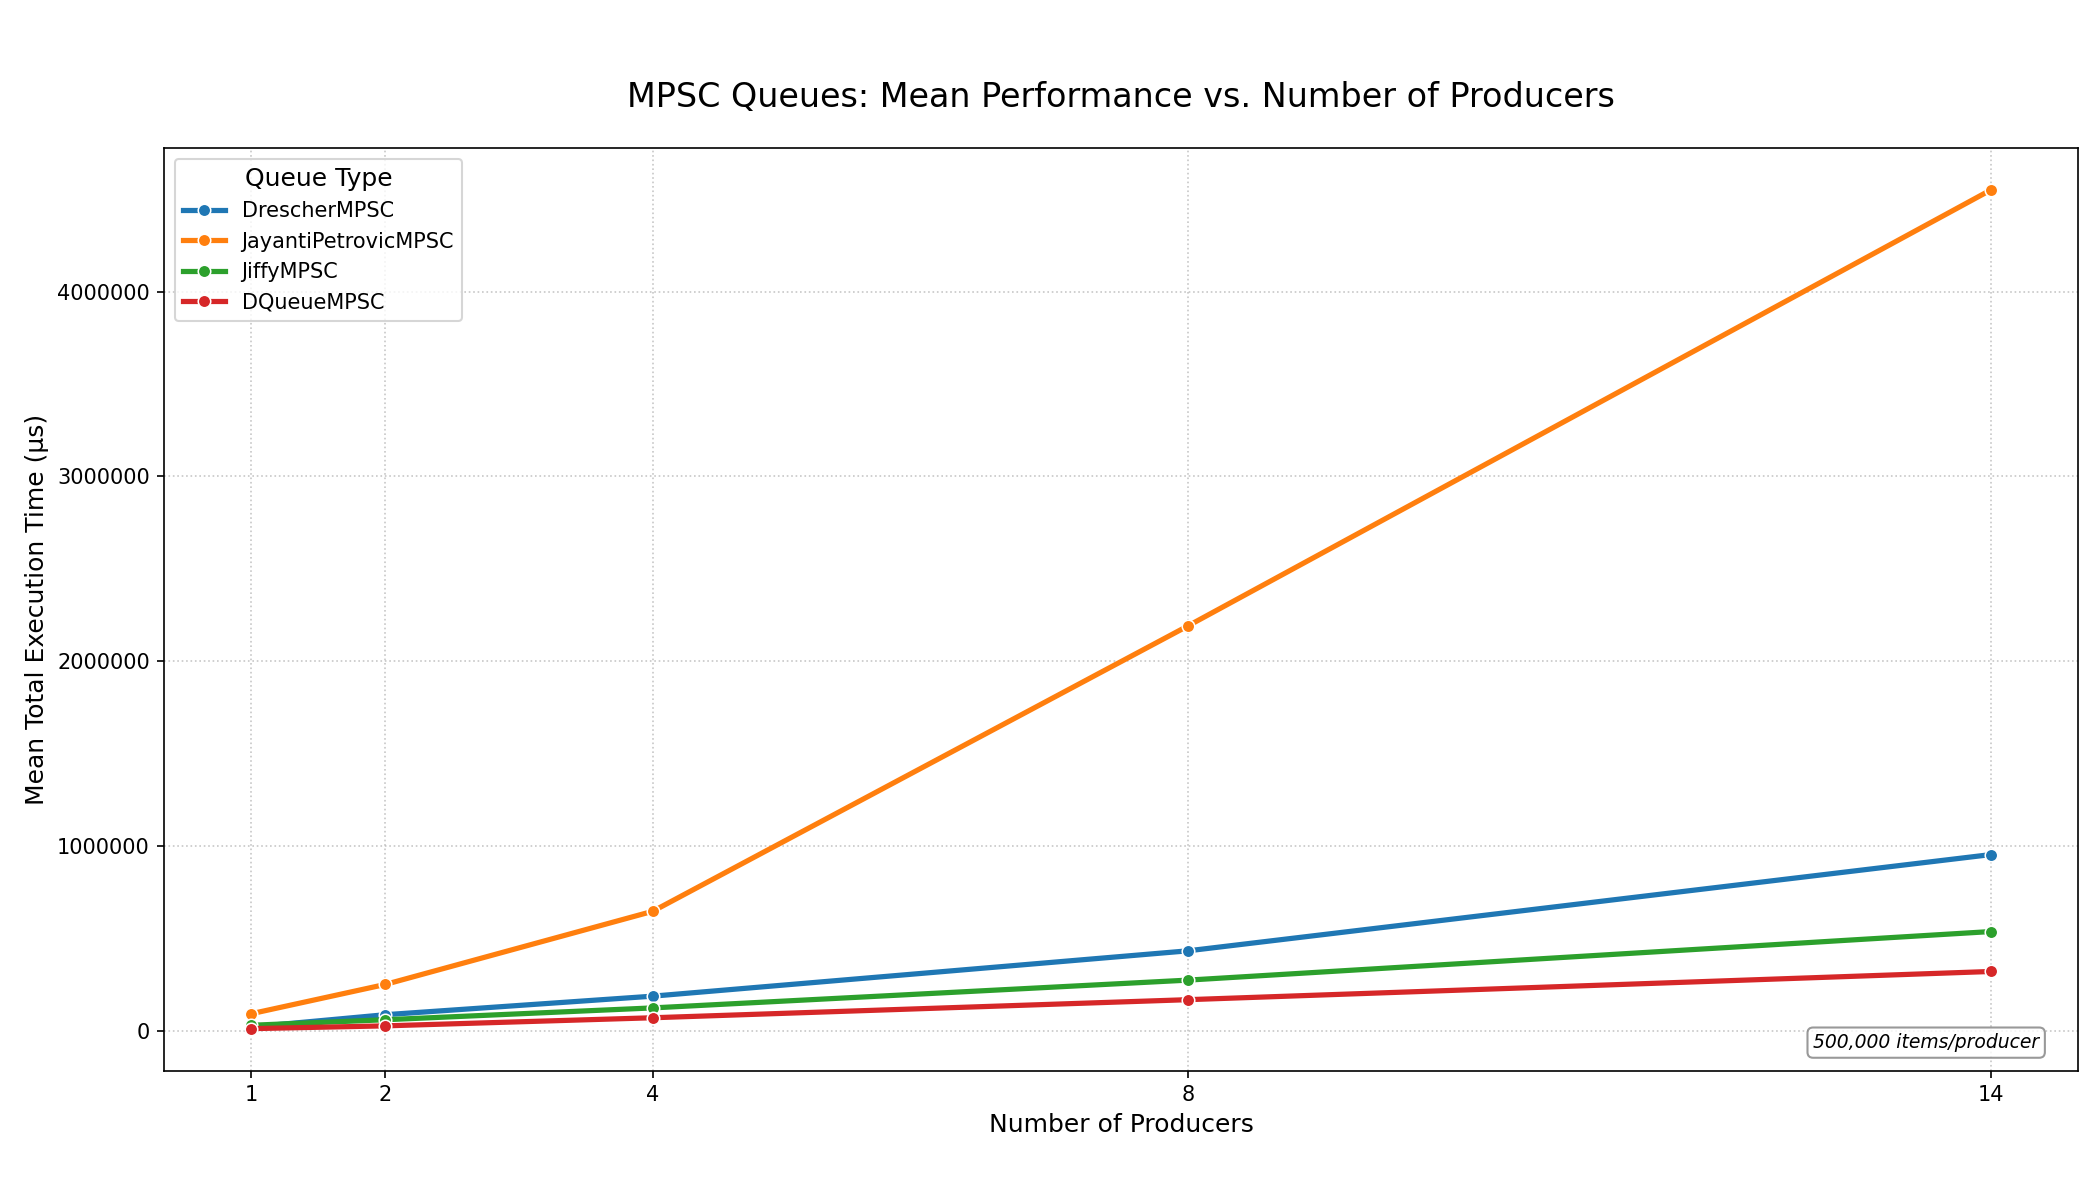
\includegraphics[width=\textwidth]{images/results/mpsc_mean_performance_vs_producers.png}
\end{figure}

DQueue had the best performance overall as producer count increased. The DQueue's local buffering mechanism effectively reduces contention by minimising synchronisation operations, as each producer accumulates items locally before batch-writing to the shared queue.

The \ac{JPQ}, despite its theoretical $O(\log n)$ complexity, showed poor practical performance being due to the overhead of maintaining the binary tree structure for timestamp propagation. This highlights the gap between theoretical complexity and real-world performance in concurrent data structures.

\begin{figure}[htb]
\centering
\caption{Violin plot showing the distribution of execution times for MPSC queue implementations with 14 producers and 1 consumer and 7,000,000 total items}
\label{fig:mpsc-violin-14p}
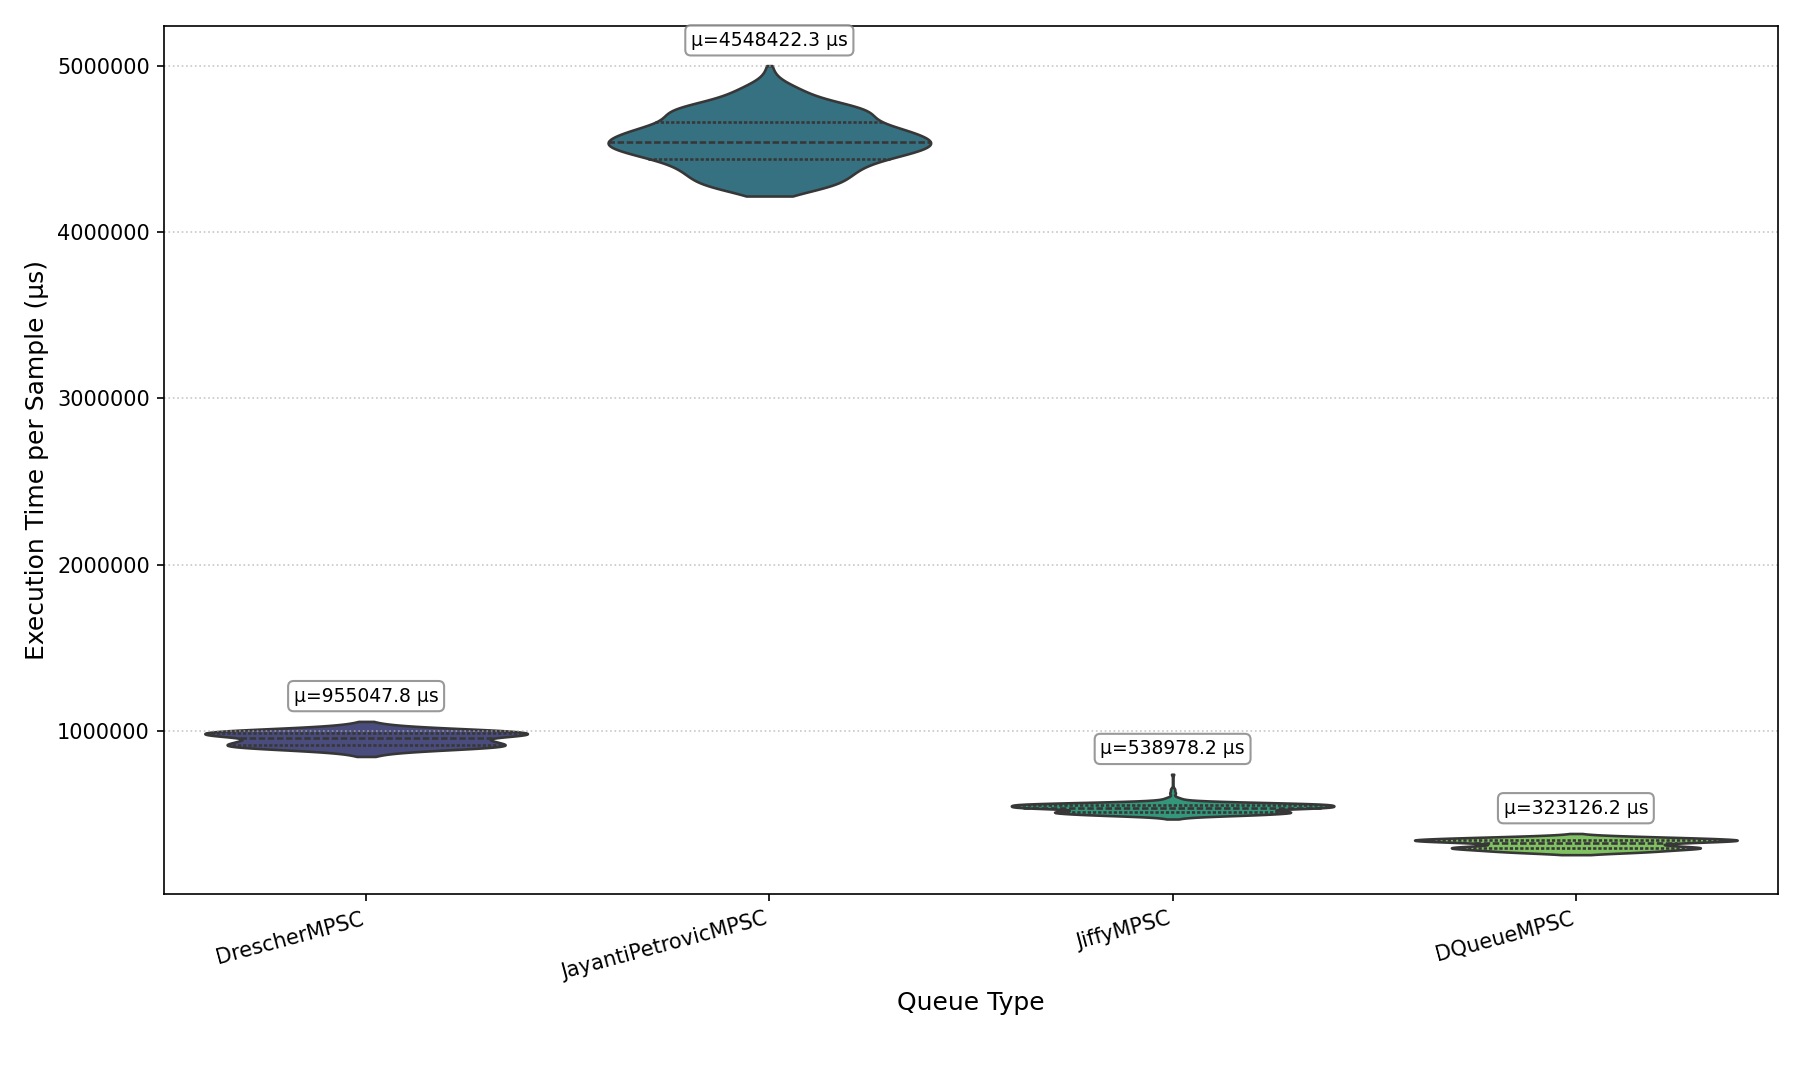
\includegraphics[width=\textwidth]{images/results/mpsc_performance_violin_14_producers.png}
\end{figure}

\cref{fig:mpsc-violin-14p} shows the performance distribution under maximum contention (14 producers). DQueue maintains a tight distribution even under high producer contention, which is also the case for lesser producer counts as seen in \cref{fig:mpsc-violin-1p,fig:mpsc-violin-2p,fig:mpsc-violin-4p,fig:mpsc-violin-8p}. This shows that DQueue's design is ensuring consistent enough performance to design hard timing constraints for \ac{HRTS}.

\subsection{\acf{SPMC} Queue Performance}
Only one native \ac{SPMC} implementation was available. So no performance comparison was made with another \ac{SPMC} queue. What was done is comparing the performance of the David queue with the best performing \ac{MPMC} queue in a \ac{SPMC} benchmark setting, to see if maybe the best performing \ac{MPMC} queue would be even better in a \ac{SPMC} setting than a native \ac{SPMC} queue. This can be seen in \cref{subsubsec:cross-spmc}.

\subsection{\acf{MPMC} Queue Performance}
The \ac{MPMC} category included six implementations tested with symmetric producer-consumer configurations. Each producer generated 170000 items. \cref{tab:mpmc-results} shows the mean performance across different producer-consumer configurations, which is again visualised as seen in \cref{fig:mpmc-mean-performance}.

\begin{table}[htb]
\centering
\caption{\ac{MPMC} Queue Performance Results (170000 items per producer)}
\label{tab:mpmc-results}
\begin{tabular}{@{}lrrrr@{}}
\toprule
Queue & 1P/1C & 2P/2C & 4P/4C & 6P/6C \\
\midrule
\ac{YMC} & 72910.8 & 72547.6 & 101541.4 & 121477.9 \\
Verma & 45690.9 & 73042.7 & 153716.8 & 229763.6 \\
FeldmanDechev & 90956.0 & 100893.5 & 150636.2 & 278037.7 \\
TurnQueue & 100150.3 & 173204.2 & 510697.0 & 971945.7 \\
KoganPetrank & 174502.6 & 285645.9 & 896079.8 & 1574045.2 \\
\ac{wCQ} & 233996.9 & 248234.3 & 350401.3 & 518476.6 \\
\bottomrule
\end{tabular}
\end{table}

\begin{figure}[htb]
\centering
\caption{Mean execution time of MPMC queue implementations as process count increases}
\label{fig:mpmc-mean-performance}
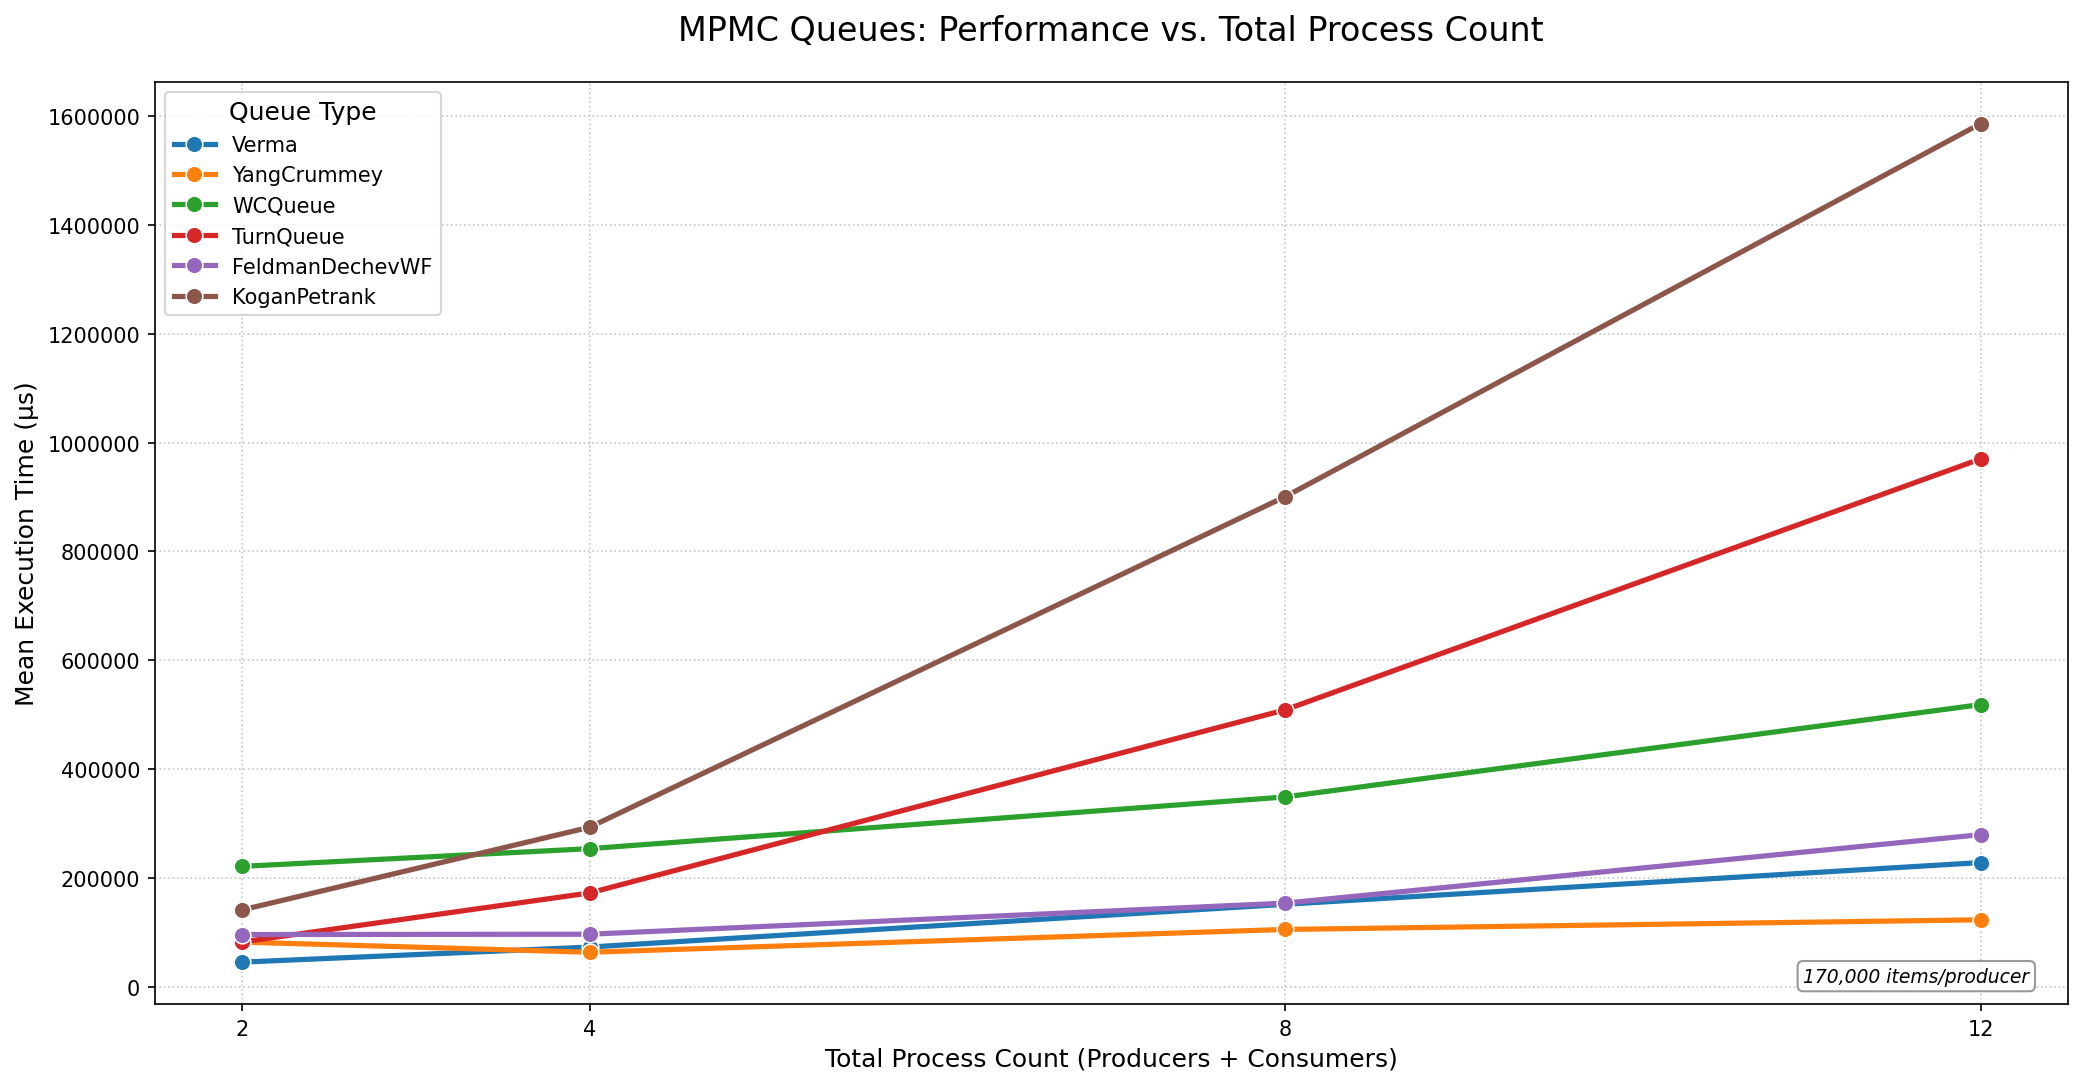
\includegraphics[width=\textwidth]{images/results/mpmc_mean_performance_vs_processes.png}
\end{figure}

The \ac{YMC} queue achieved the best overall performance with 72910.8 $\mu$s for 1 producer and 1 consumer, 72547.6 $\mu$s for 2 producers and 2 consumers, and scaling to 121477.9 $\mu$s for 6 producers and 6 consumers. Its performance remained relatively stable across different configurations, demonstrating its efficiency in handling multiple producers and consumers.

What can be observed is that the Verma queue has better performance in the 1P/1C case with a mean performance of 45690.9 $\mu$s than \ac{YMC}. The reason for that is most probably, because even in the 1P/1C case there is still an active dedicated helper thread that is used to help the producer and consumer processes.

\begin{figure}[htb]
\centering
\caption{Violin plot showing the distribution of execution times for MPMC queue implementations with 6 producers and 6 consumers an 1,020,000 total items}
\label{fig:mpmc-violin-6p6c}
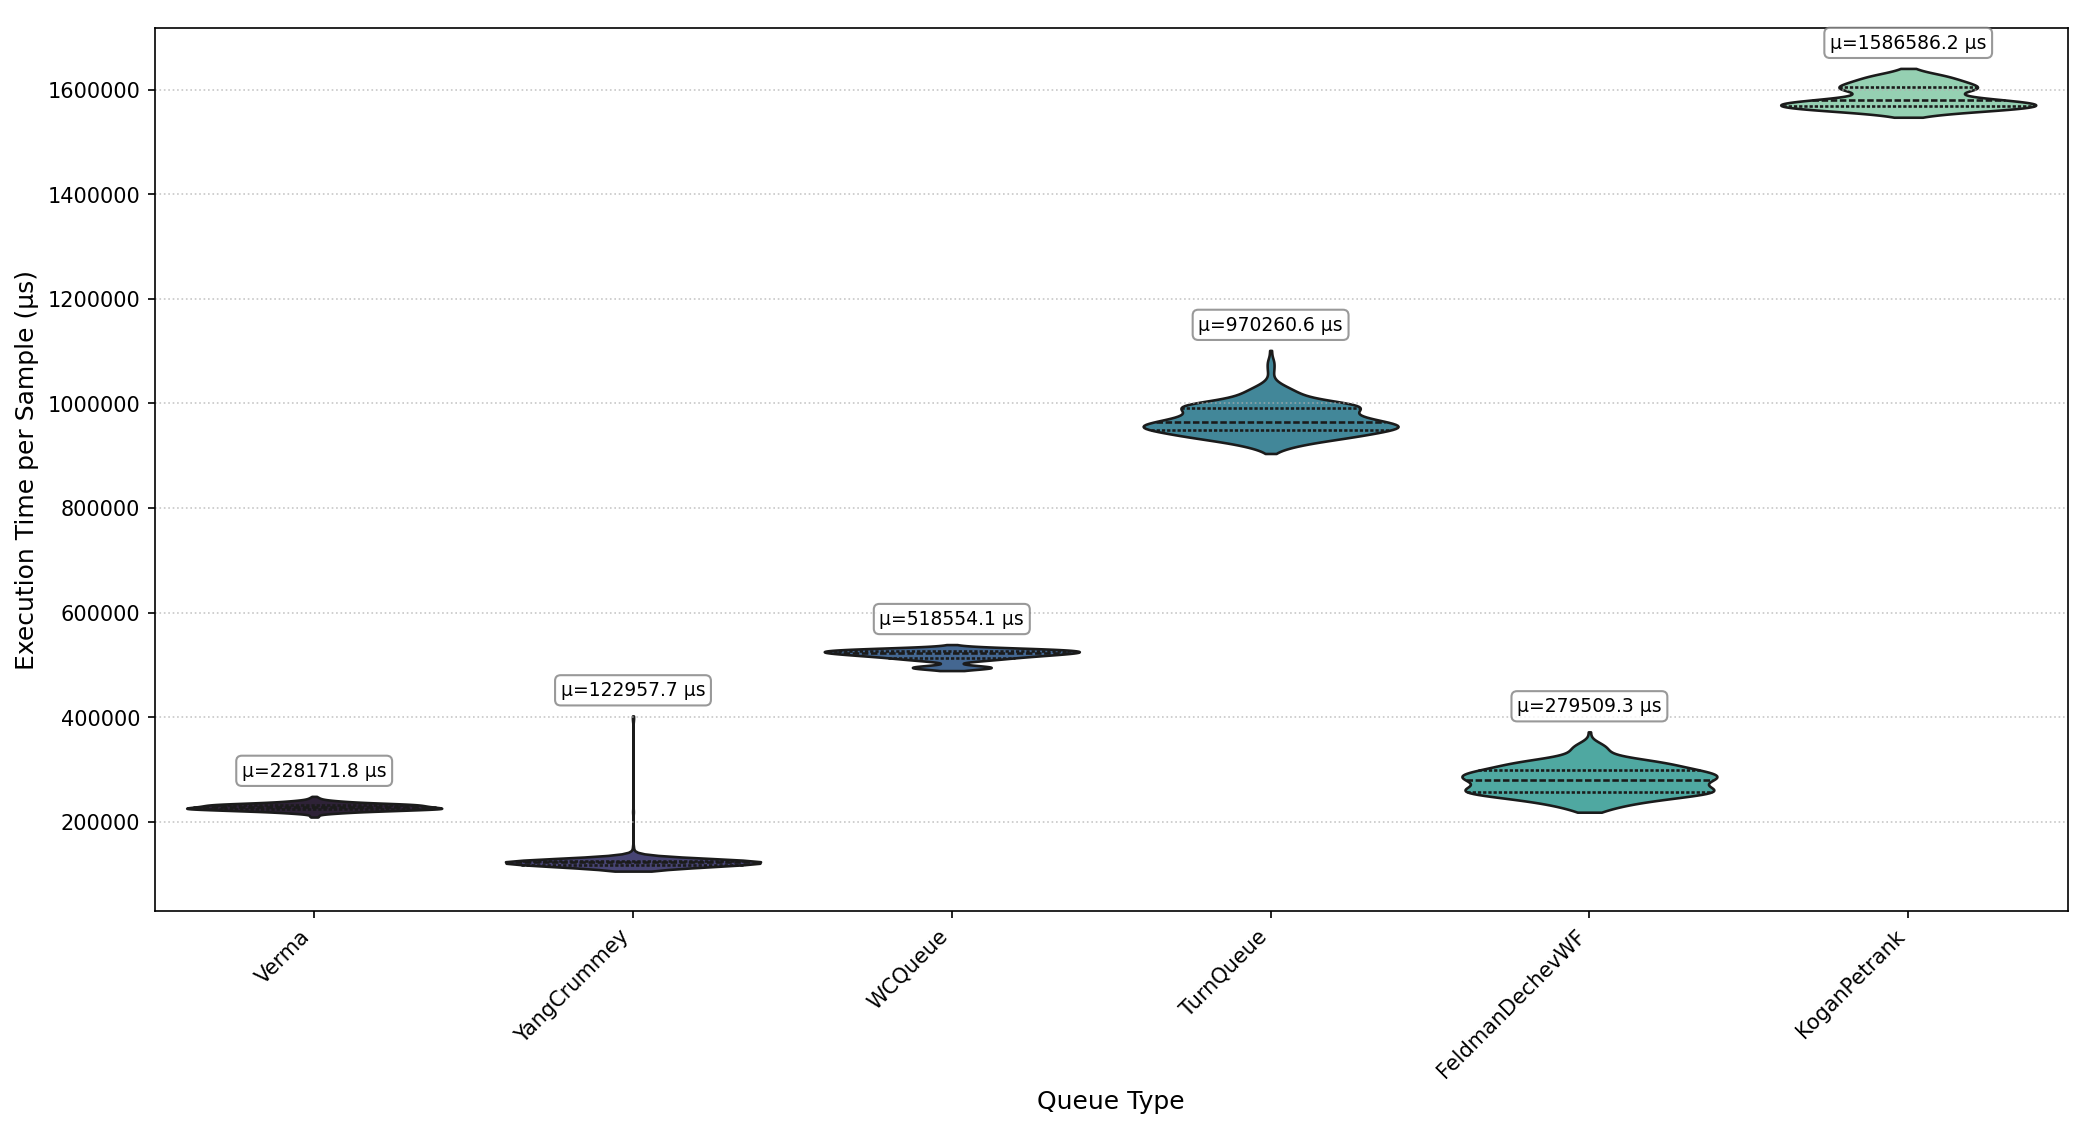
\includegraphics[width=\textwidth]{images/results/mpmc_performance_violin_6P_6C.png}
\end{figure}

\cref{fig:mpmc-violin-6p6c} illustrates the performance distribution under symmetric high contention (6P/6C). The \ac{YMC} queue demonstrates that its performance stays consistent with minimal variance, even in lesser producer and consumer counts as seen in \cref{fig:mpmc-violin-2p2c,fig:mpmc-violin-4p4c}, indicating predictable performance beneficial to define tight timing constraints for \ac{HRTS}. The only exception is the 1P/1C case, where the performance distribution is more spread out, as seen in \cref{fig:mpmc-violin-1p1c} indicating that \ac{YMC} is not as optimised for low contention scenarios as it is for high contention scenarios. The Verma queue has consistent performance over all process counts, but with a higher mean execution time than \ac{YMC}. So for \ac{HRTS} which requires predictability Verma queue could be a better choice even though it is not the fastest queue in the \ac{MPMC} category.

\subsection{Cross-Category Performance Comparison}
To determine whether specialised queues for each contention category are necessary, cross-category benchmarks were conducted comparing the best performers from each category against queues from other categories. The specialised queues for their respective contention scenarios were called native in each cross-category benchmark. The results are summarised in the following subsections.


\subsubsection{Best Queue for \ac{SPSC} Scenarios}
\cref{tab:best-spsc} compares the native \ac{SPSC} winner (\ac{BLQ}) against the best queues from other categories operating in \ac{SPSC} mode with 300000 items.

\begin{table}[htb]
\centering
\caption{Cross-Category Performance in \ac{SPSC} Configuration (300000 items)}
\label{tab:best-spsc}
\begin{tabular}{@{}lrr@{}}
\toprule
Queue (Category) & Mean Time ($\mu$s) & Relative to \ac{BLQ} \\
\midrule
\ac{BLQ} (Native SPSC) & 3625.7 & 1.00x \\
DQueue (MPSC as SPSC) & 7638.9 & 2.11x \\
David (SPMC as SPSC) & 21207.3 & 5.85x \\
\ac{YMC} (MPMC as SPSC) & 36170.9 & 9.98x \\
\bottomrule
\end{tabular}
\end{table}

The native \ac{SPSC} queue with a mean performance of $3625.7\mu$s outperformed all others, being 2.11x faster than DQueue and nearly 10x faster than \ac{YMC}. This demonstrates that specialised \ac{SPSC} algorithms provide benefits when contention is limited to a single producer and consumer pair. \cref{fig:cross-spsc-violin} visualises this again.

\begin{figure}[htb]
\centering
\caption{Violin plot showing performance distribution of different queue categories operating in an \ac{SPSC} setting with 300,000 total items}
\label{fig:cross-spsc-violin}
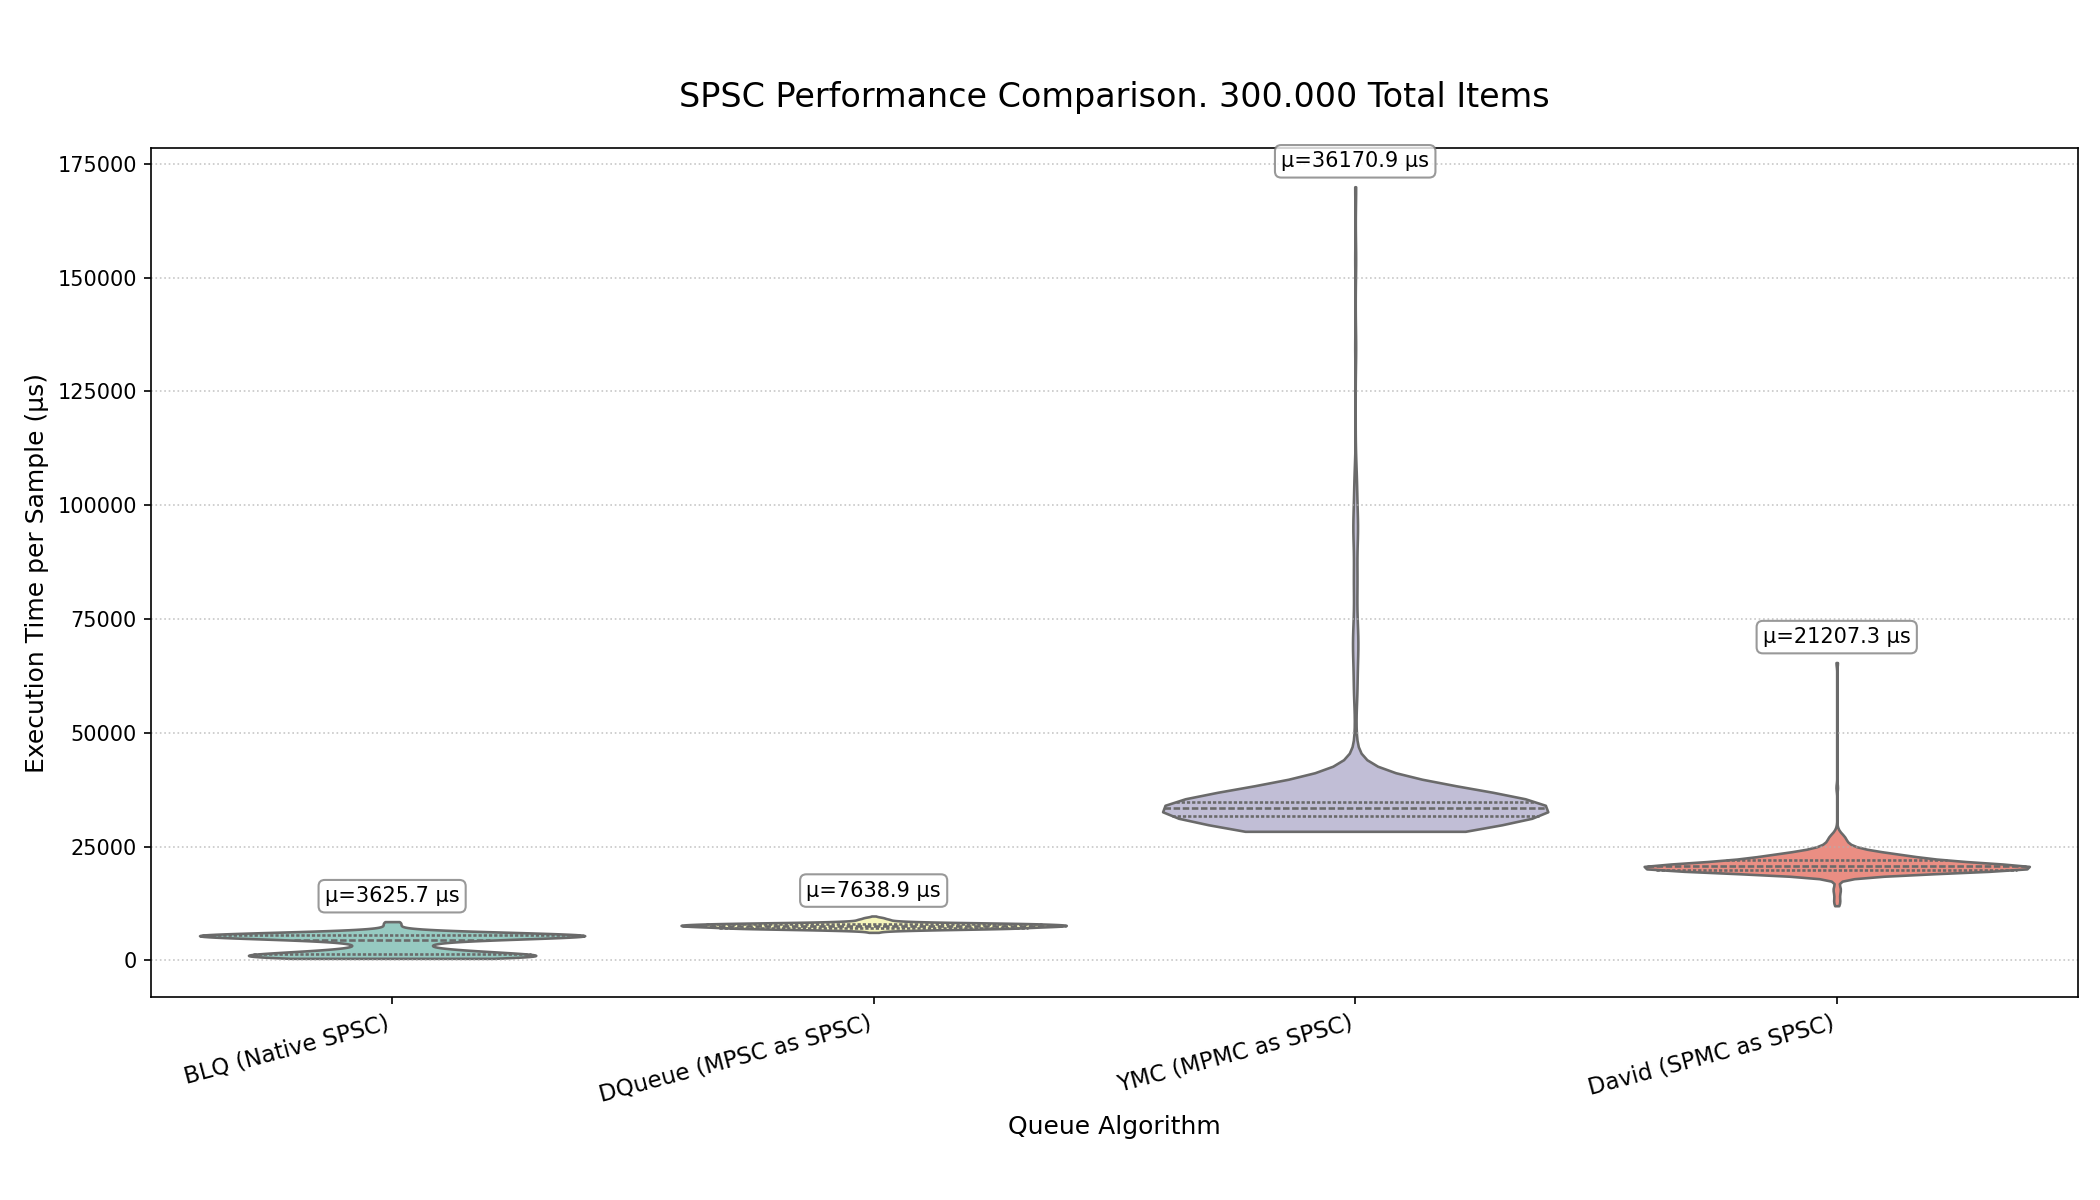
\includegraphics[width=\textwidth]{images/results/best_algorithms_in_spsc_performance.png}
\end{figure}

\subsubsection{Best Queue for \ac{MPSC} Scenarios}
Comparing the native \ac{MPSC} winner DQueue against \ac{YMC} operating in an \ac{MPSC} setting reveals similar patterns, as shown in \cref{tab:best-mpsc} visualised in \cref{fig:cross-mpsc-mean}.

\begin{table}[htb]
\centering
\caption{Cross-Category Performance in \ac{MPSC} Configuration (100000 items per producer)}
\label{tab:best-mpsc}
\begin{tabular}{@{}lrrr@{}}
\toprule
Producers & DQueue (Native \ac{MPSC}) & \ac{YMC} (as \ac{MPSC}) & Relative to DQueue \\
& Time ($\mu$s) & Time ($\mu$s) & \\
\midrule
1 & 2102.7 & 13075.6 & 6.22x \\
2 & 7081.9 & 19650.4 & 2.77x \\
4 & 16588.1 & 39848.3 & 2.40x \\
8 & 36197.5 & 84092.5 & 2.32x \\
14 & 72788.4 & 168854.4 & 2.32x \\
\bottomrule
\end{tabular}
\end{table}

DQueue outperformed \ac{YMC} across all producer counts, with the performance gap decreasing from 6.22x at 1 producer to 2.32x at 14 producers. The native \ac{MPSC} implementation maintains its advantage due to its optimised local buffering mechanism that reduces synchronisation overhead. \ac{YMC} has overhead from its additional consumer synchronisation mechanisms, which are not needed in an \ac{MPSC} setting.

\begin{figure}[htb]
\centering
\caption{Mean execution time comparison of DQueue (native MPSC) vs YMC (as MPSC) across different producer counts}
\label{fig:cross-mpsc-mean}
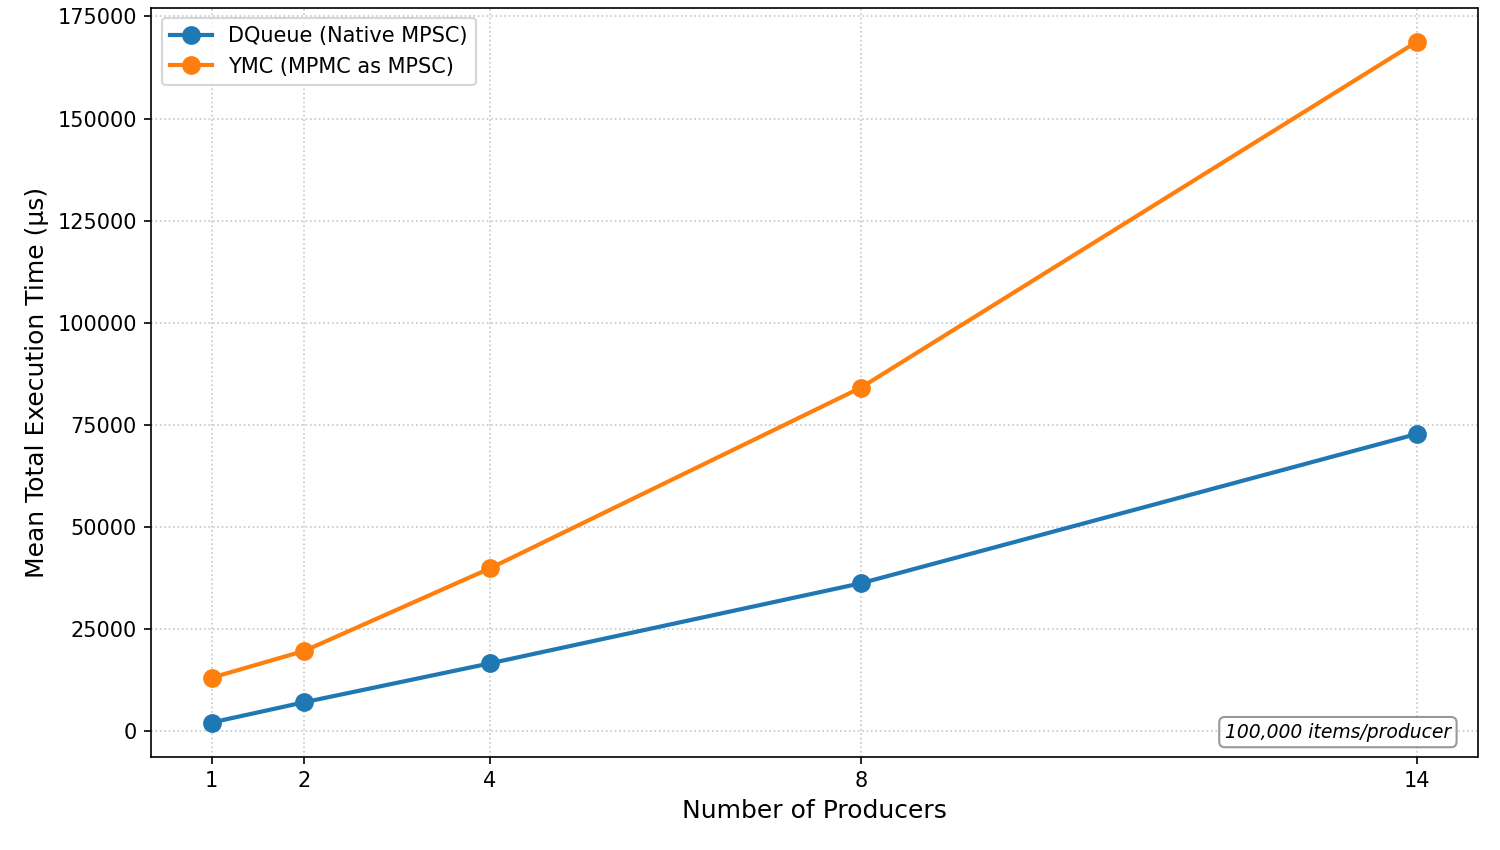
\includegraphics[width=\textwidth]{images/results/best_in_mpsc_mean_performance_vs_producers.png}
\end{figure}

\begin{figure}[htb]
\centering
\caption{Violin plot showing the distribution of execution times for cross-category MPSC comparison with 14 producers and 1 consumer and 1,400,000 total items}
\label{fig:cross-mpsc-violin-14p}
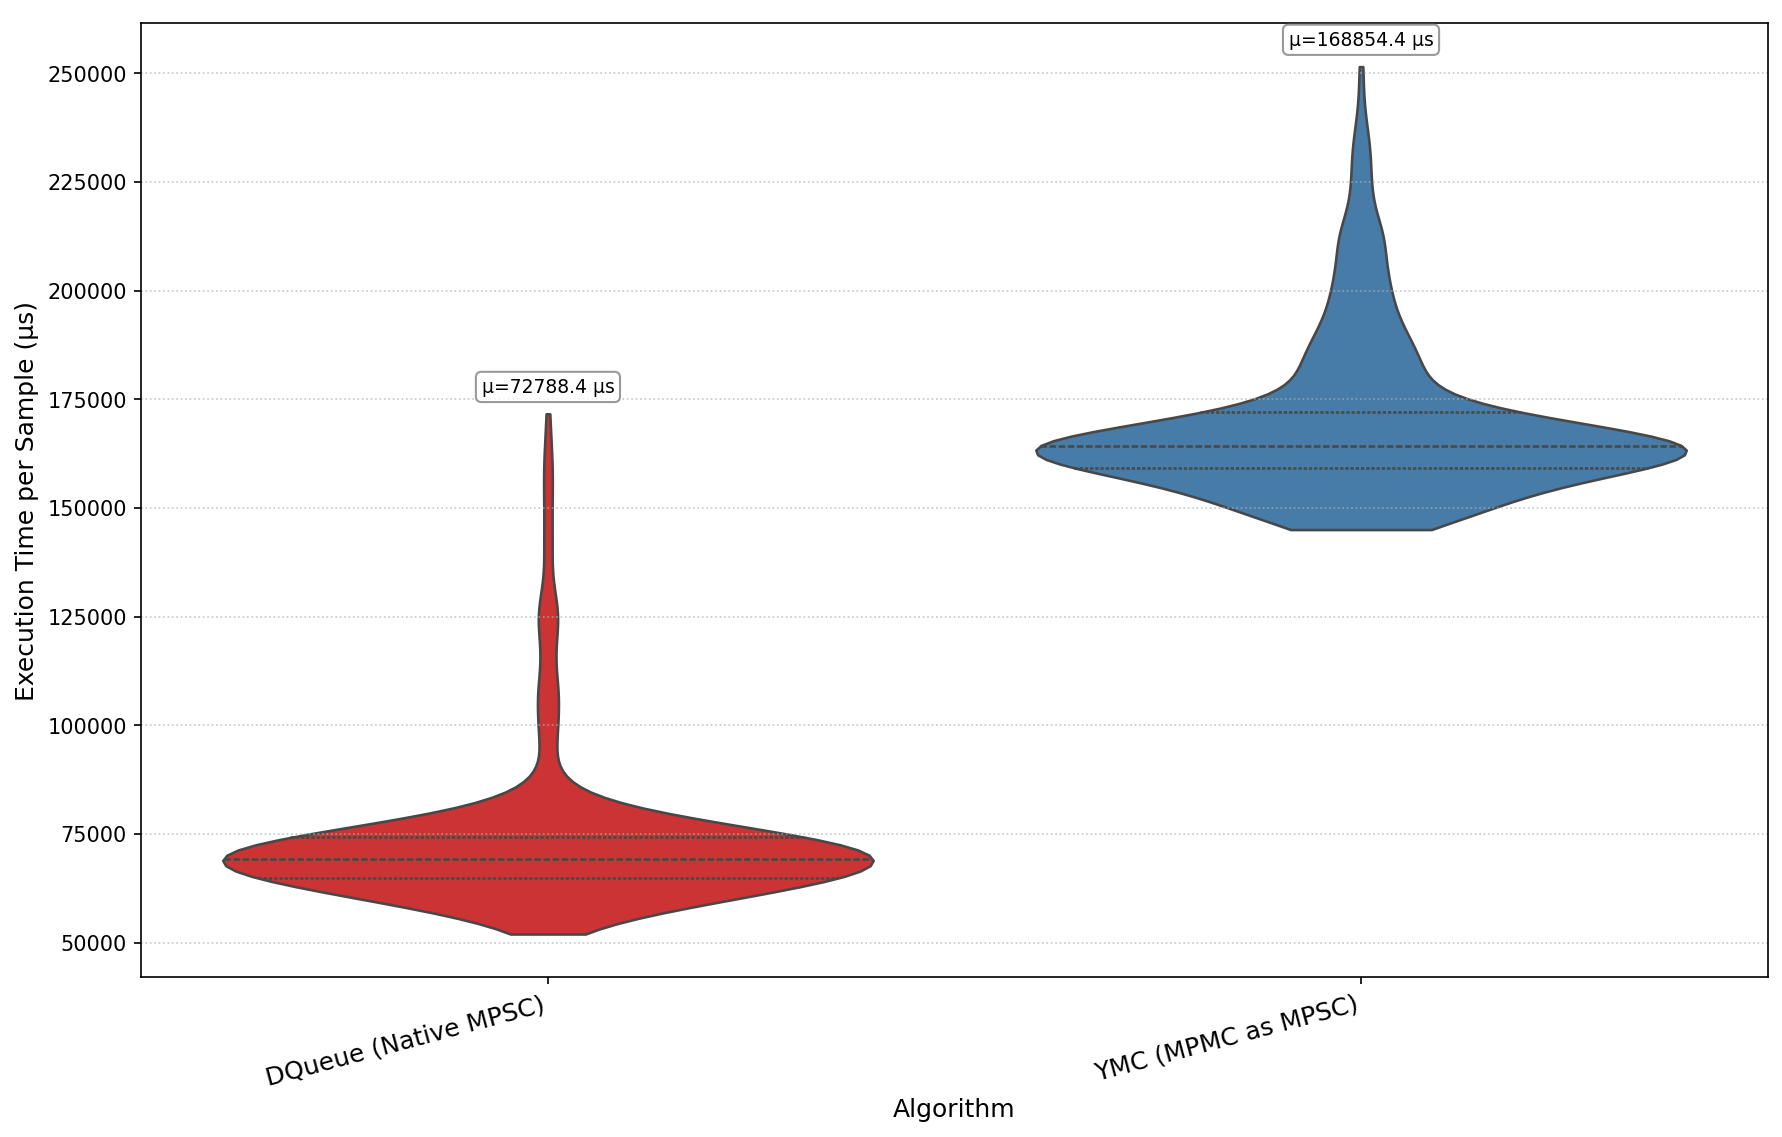
\includegraphics[width=\textwidth]{images/results/best_in_mpsc_performance_violin_14P1C.png}
\end{figure}

\cref{fig:cross-mpsc-violin-14p} illustrates the performance distribution comparison between DQueue (native MPSC) and \ac{YMC} (operating as MPSC) under maximum producer contention (14 producers). DQueue shows slightly better consistency whilst performing faster than \ac{YMC}, showing that also in \ac{MPSC} settings specialised queues are better than more general \ac{MPMC} queues. The same goes too for lesser producer counts as seen in \cref{fig:cross-mpsc-violin-1p,fig:cross-mpsc-violin-2p,fig:cross-mpsc-violin-4p,fig:cross-mpsc-violin-8p}.

\subsubsection{Best Queue for \ac{SPMC} Scenarios}\label{subsubsec:cross-spmc}
The native \ac{SPMC} implementation (David) was compared against \ac{YMC} in \ac{SPMC} mode, as presented in \cref{tab:best-spmc}.

\begin{table}[htb]
\centering
\caption{Cross-Category Performance in \ac{SPMC} Configuration (100000 items per consumer)}
\label{tab:best-spmc}
\begin{tabular}{@{}lrrr@{}}
\toprule
Consumers & David (Native \ac{SPMC}) & \ac{YMC} (as \ac{SPMC}) & Relative to David \\
& Time ($\mu$s) & Time ($\mu$s) & \\
\midrule
1 & 2754.4 & 16696.0 & 6.06x \\
2 & 8222.4 & 24220.6 & 2.95x \\
4 & 17243.9 & 44368.2 & 2.57x \\
8 & 37756.0 & 96410.1 & 2.55x \\
14 & 71305.7 & 225931.3 & 3.17x \\
\bottomrule
\end{tabular}
\end{table}

Similar to the \ac{MPSC} results, the specialised David queue significantly outperformed \ac{YMC}, maintaining a 2.5-6x performance advantage across different consumer counts. The native \ac{SPMC} algorithm's two-dimensional array design with row jumping proves to be faster than the general-purpose \ac{MPMC} approach.

\begin{figure}[htb]
\centering
\caption{Violin plot showing the distribution of execution times for \ac{SPMC} implementations with 1 producer and 14 consumers and 1,400,000 total items}
\label{fig:spmc-violin-14c}
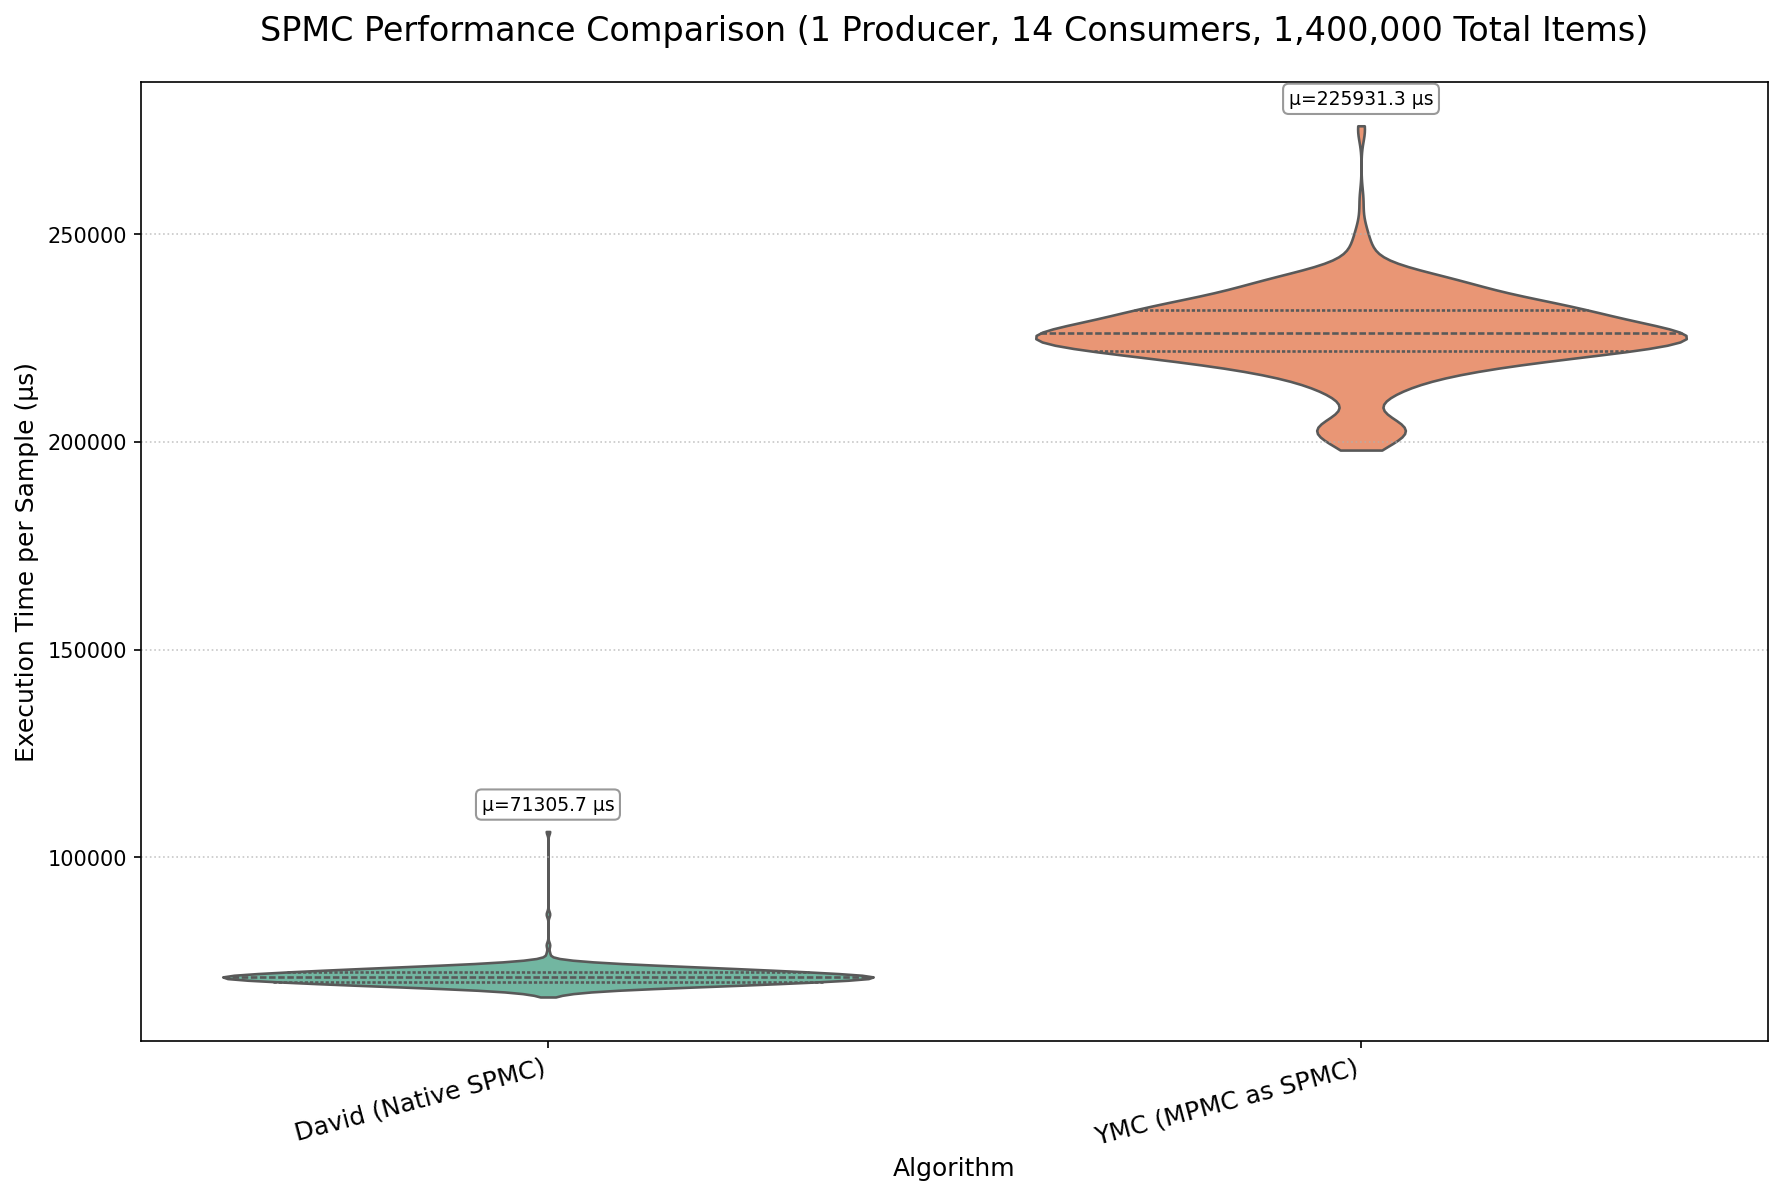
\includegraphics[width=\textwidth]{images/results/best_in_spmc_performance_violin_1P14C.png}
\end{figure}

The violin plot in \cref{fig:spmc-violin-14c} demonstrates the performance distribution under maximum consumer contention. The David queue shows more consistent performance with a tighter distribution whilst being faster compared to \ac{YMC} operating in SPMC mode, confirming again specialised queues are the better choice. Also here the same can be said for lesser consumer counts as seen in \cref{fig:cross-spmc-violin-1c,fig:cross-spmc-violin-2c,fig:cross-spmc-violin-4c,fig:cross-spmc-violin-8c}.

\begin{figure}[htb]
\centering
\caption{Mean execution time comparison of David (native SPMC) vs YMC (as SPMC) across different consumer counts}
\label{fig:cross-spmc-mean}
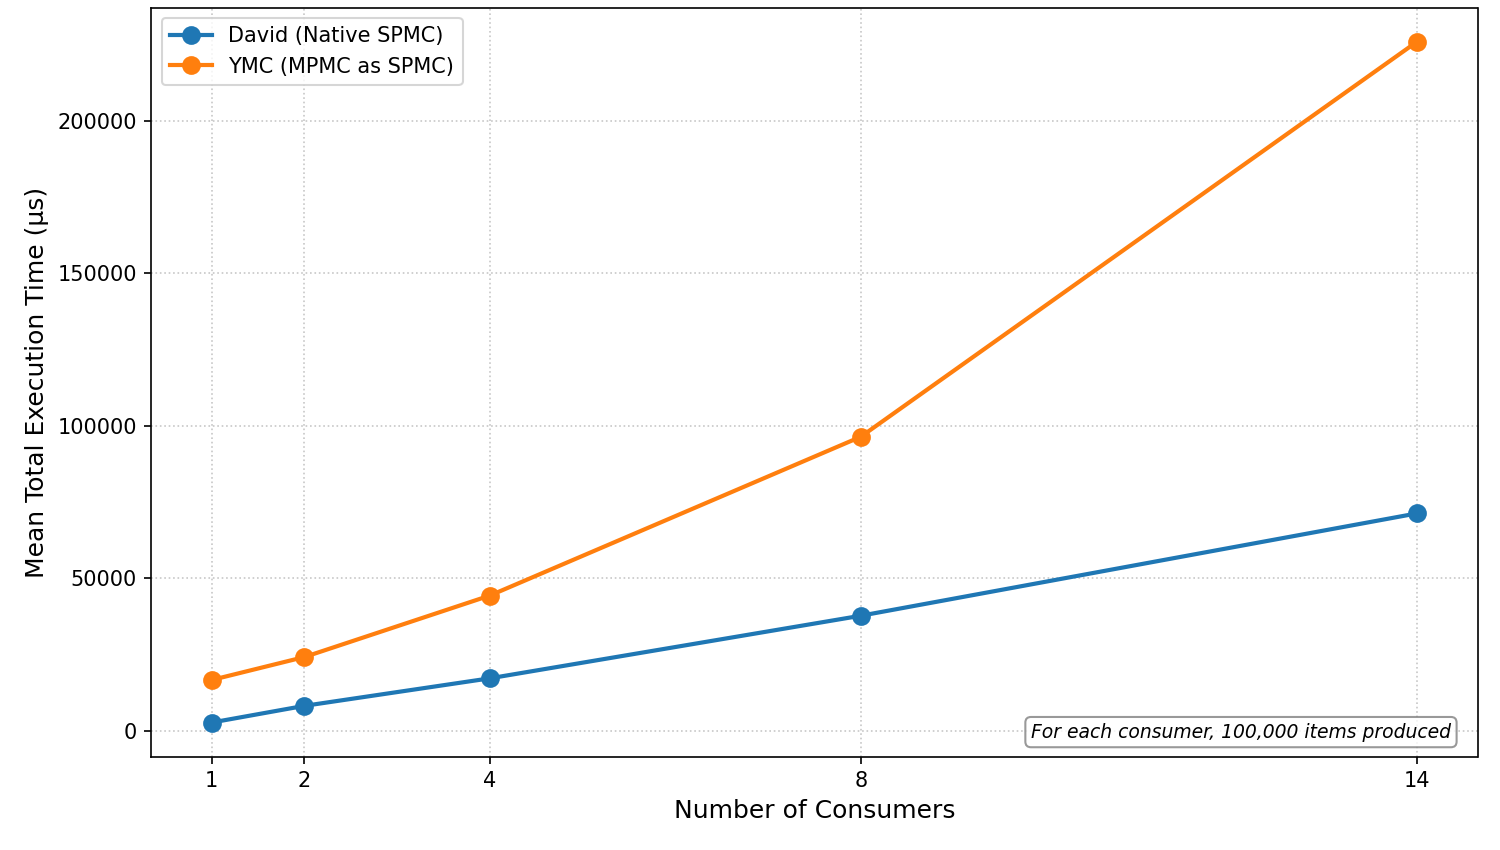
\includegraphics[width=\textwidth]{images/results/best_in_spmc_mean_performance_vs_consumers.png}
\end{figure}